\chapter{Mathematical Background}\label{math}
\section{Introduction}
Discontinuous Galerkin finite element method is an amalgamation of the element based Galerkin schemes and
the finite volume method. It is a compact, higher-order accurate scheme where the solution can be 
discontinuous between two elements.
The DG scheme requires the physical domain ($\Omega$) discretized with $Ne$ finite elements (written as $\Omega^k$). 
The finite element cells are assumed to be one of the following types.
\begin{enumerate}
	\item Hexahedral ($8$ edges, $8$ nodes, $6$ faces)
	\item Tetrahedral ($6$ edges, $4$ nodes, $4$ faces)
	\item Prism ($9$ edges, $6$ nodes, $5$ faces)
	\item Pyramid ($8$ edges, $5$ nodes, $5$ faces)
\end{enumerate}
The solution is assumed to be continuous (along with continuous derivatives depending on the governing equations) inside 
the element. However, the solution can be discontinuous at the edges and faces. The value of the conserved variable (and 
the numerical fluxes) at the faces and edges are found out by solving the Riemann problem which arises because of the 
discontinuity. 

The DG method essentially starts with the `variational' formulation of the problem. Consider a 
differential equation given by,
\begin{equation}\label{diffeqn}
	\mathbf{L}(u) = f(u),  u\in{H^1(\Omega)}
\end{equation}
(and suitable boundary conditions, not mentioned here).
For example, $\mathbf{L} = \frac{d}{dx}$ and $f(u) = u$ results in,
\begin{equation}\label{diffeqn_ex1}
	\frac{du}{dx} = u
\end{equation}
We will be using the general notation given by equation \ref{diffeqn} henceforth.
Then, if $u^k$ is the approximate solution inside of the element, then instead of the solving equation \ref{diffeqn}
with $u^k$, we solve the following variational formulation of equation \ref{diffeqn}.
\begin{equation}\label{diffeqnvr}
	\int_{\Omega_k} \phi \mathbf{L}(u^k) d\Omega = 	\int_{\Omega_k} \phi f(u^k) d\Omega
\end{equation}
$\phi$ is the test function. The approximate solution $u^k$ is obtained by polynomial approximation of $u$ inside $\Omega^k$.
A modal interpolation (basis functions consisting of modes, i.e. frequencies) or a nodal interpolation (basis functions
consist of the cardinal polynomials such as the Lagrange polynomials) can be used for this. 
In the DG methods, the basis functions serve as the test functions. 
The integrations in equation \ref{diffeqn_ex1} are solved numerically using quadrature formulas. 
The resulting algebraic system is solved iteratively (or ODE is solved numerically if time dependant).
This process is repeated till convergence (for steady state
problems) or till the final time is reached (for transient problems). 
It is easier to solve the problem on a reference cell (canonical element) and then map the solution on to the physical cell.
This requires a mapping to be defined between the reference cell and the physical cell.
Based on this general process, the following mathematical concepts are revised in this chapter.
\begin{enumerate}
	\item Mapping functions (Jacobian ($\mathbf{J}$) of transformation, inverse Jacobian ($\mathbf{J}^{-1}$) and ($|\mathbf{J}|$))
	\item Modal and nodal basis functions  
	\item Polynomial interpolation and differentiation
	\item Numerical quadrature (integration)
	\item Cell matrices (Vandermonde matrix, Mass matrix, differentiation matrix and flux matrix)
	\item Other mathematical functions 
\end{enumerate}
The discussion is kept brief and concise and only those concepts concerned with MEAN-DG are discussed. 
The user is encouraged to go through the references for in-depth theory of DG schemes.

\begin{note}
	We use the c++ style indexing. i.e. indices start at $0$ (not $1$).
\end{note}

\section{Mapping on the Reference Element}
Corresponding to each physical cell, there exists a canonical (reference) element.
The physical cell is expressed in terms of the physical coordinate system $(x,y,z)$. The reference coordinate system is
written in terms of  $(r,s,t)$. 
Thus, each of the physical coordinates can be written in terms of the $(r,s,t)$ coordinate system. In the code, we 
describe the physical coordinate system as $XYZ$, and the reference system as $RST$. 
The mapping from the physical coordinate system to the reference coordinate system is characterized by the Jacobian of 
transformation $\mathbf{J}$. 
In this section, we describe the Jacobian of transformation for the four types of the cells.

\subsection{Hexahedral cells}
Hexahedral, or Hex in short, cells are mapped to a cube in 3D. The Hex cell has $8$ nodes given by the array,
$\left((x_0,y_0,z_0), (x_1, y_1, z_1), ... ,(x_7,y_7,z_7)\right)$.
We define the linear shape functions on the reference element as follows:
\begin{equation}\label{shape0}
	N_0 = \frac{1}{8} (1-r) (1-s) (1-t), \hspace{5mm} \{r,s,t \in V | \forall v\in V \subset  {\mathbb{R}} , ~ v \in [-1,1]\}
\end{equation}
\begin{equation}\label{shape1}
	N_1 = \frac{1}{8} (1+r) (1-s) (1-t) 
\end{equation}
\begin{equation}\label{shape2}
	N_2 = \frac{1}{8} (1+r) (1+s) (1-t) 
\end{equation}
\begin{equation}\label{shape3}
	N_3 = \frac{1}{8} (1-r) (1+s) (1-t) 
\end{equation}
\begin{equation}\label{shape4}
	N_4 = \frac{1}{8} (1-r) (1-s) (1+t) 
\end{equation}
\begin{equation}\label{shape5}
	N_5 = \frac{1}{8} (1+r) (1-s) (1+t) 
\end{equation}
\begin{equation}\label{shape6}
	N_6 = \frac{1}{8} (1+r) (1+s) (1+t) 
\end{equation}
\begin{equation}\label{shape7}
	N_7 = \frac{1}{8} (1-r) (1+s) (1+t) 
\end{equation}

The mapping then is simply given as,

\begin{equation}\label{mapx}
	x(r,s,t) = \sum_{i=0}^7 N_i x_i
\end{equation}

\begin{equation}\label{mapy}
	y(r,s,t) = \sum_0^7 N_i y_i
\end{equation}

\begin{equation}\label{mapz}
	z(r,s,t) = \sum_0^7 N_i z_i
\end{equation}

\begin{definition}\label{Jacobian}
	The Jacobian of transformation ($\mathbf{J}$) is defined as :
	\begin{equation}\label{J}
		{\setstretch{2}
		\mathbf{J} = \left[\begin{array}{c c c}
			\frac{\partial x}{\partial r} & \frac{\partial x}{\partial s} &  \frac{\partial x}{\partial t} \\
			\frac{\partial y}{\partial r} & \frac{\partial y}{\partial s} &  \frac{\partial y}{\partial t} \\
			\frac{\partial z}{\partial r} & \frac{\partial z}{\partial s} &  \frac{\partial z}{\partial t} \\
												                   \end{array} \right]
			= \left[\begin{array}{c c c}
				J_{00} & J_{01}  & J_{02}   \\
				J_{10} & J_{11}  & J_{12}   \\
				J_{20} & J_{21}  & J_{22}   \\
												                   \end{array} \right]
	        }
	\end{equation}
\end{definition}
The partial derivatives in equation \ref{J} can be easily computed from equations \ref{shape0}-\ref{shape7} and \ref{mapx}, \ref{mapy}, \ref{mapz}.
In the code, the above implementation is found in Cell.cpp.
\begin{verbatim} 
Cell::calculateJacobian3DTensor(double r,double s,double t) 
\end{verbatim}
\begin{note}
	The first name indicates the name of the class (Cell), the second symbol (::) indicates the scope (in this case, indicating
	'belongs to Cell' the third name is the name of the class method (calculateJacobian3DTensor) and terms in the bracket being
	arguments passed to this function.
\end{note}
It is to be noted that the name `Tensor' in the above function indicates that the functional space for a Hex cell is 
obtained by a tensor product (outer product) of 1D functional spaces.

The inverse of the Jacobian is found out by the standard process of inversion of a matrix.

\begin{equation}\label{JInv}
	{\setstretch{2}
	\mathbf{J^{-1}} = \left[\begin{array}{c c c}
		\frac{\partial r}{\partial x} & \frac{\partial r}{\partial y} &  \frac{\partial r}{\partial z} \\
		\frac{\partial s}{\partial x} & \frac{\partial s}{\partial y} &  \frac{\partial s}{\partial z} \\
		\frac{\partial t}{\partial x} & \frac{\partial t}{\partial y} &  \frac{\partial t}{\partial z} \\
											                   \end{array} \right]
        }
\end{equation}
These are given as:
\begin{equation}\label{metricTerms00}
	\frac{\partial r}{\partial x} = \frac{1}{|{\mathbf{J}}|} \left( J_{22}J_{11} - J_{21}J_{12}\right)
\end{equation}
\begin{equation}\label{metricTerms01}
	\frac{\partial r}{\partial y} = \frac{-1}{|{\mathbf{J}}|} \left( J_{22}J_{01} - J_{21}J_{02}\right)
\end{equation}
\begin{equation}\label{metricTerms02}
	\frac{\partial r}{\partial z} = \frac{1}{|{\mathbf{J}}|} \left( J_{12}J_{01} - J_{11}J_{02}\right)
\end{equation}
\begin{equation}\label{metricTerms10}
	\frac{\partial s}{\partial x} = \frac{-1}{|{\mathbf{J}}|} \left( J_{22}J_{10} - J_{20}J_{12}\right)
\end{equation}
\begin{equation}\label{metricTerms11}
	\frac{\partial s}{\partial y} = \frac{1}{|{\mathbf{J}}|} \left( J_{22}J_{00} - J_{20}J_{02}\right)
\end{equation}
\begin{equation}\label{metricTerms12}
	\frac{\partial s}{\partial z} = \frac{-1}{|{\mathbf{J}}|} \left( J_{12}J_{00} - J_{10}J_{02}\right)
\end{equation}
\begin{equation}\label{metricTerms20}
	\frac{\partial t}{\partial x} = \frac{1}{|{\mathbf{J}}|} \left( J_{21}J_{10} - J_{20}J_{11}\right)
\end{equation}
\begin{equation}\label{metricTerms21}
	\frac{\partial t}{\partial y} = \frac{-1}{|{\mathbf{J}}|} \left( J_{21}J_{00} - J_{20}J_{01}\right)
\end{equation}
\begin{equation}\label{metricTerms22}
	\frac{\partial t}{\partial z} = \frac{1}{|{\mathbf{J}}|} \left( J_{11}J_{00} - J_{10}J_{01}\right)
\end{equation}
where, the determinant of the Jacobian $|{\mathbf{J}}|$ is calculated as:
\begin{equation}\label{detJ}
	|{\mathbf{J}}| = J_{00} (J_{22}J_{11} - J_{21}J_{12}) - J_{01} (J_{22}J_{10} - J_{20}J_{12})  + J_{02} (J_{21}J_{10} - J_{20}J_{11}) 
\end{equation}
The inverse of Jacobian is implemented in 
\begin{verbatim} 
Cell::calculateInverseJacobianMatrix3DTensor(arguments) 
\end{verbatim}

\begin{note}
	The inverse of Jacobian is called as {\bf dRST\_by\_dXYZ} in the code. Each cell stores these matrices for all the quadrature
	points within that cell. The metric terms given by \ref{metricTerms00}--\ref{metricTerms22} 
	are used in computations involving derivatives as seen in the subsequent sections and chapters.
\end{note}
The inverse Jacobian is stored for all the quadrature points for all the cells. It is an attribute of the cell
(i.e. Cell::dRST\_by\_dXYZ) and has dimensions $nQuad \times 3 \times 3$.

{\bf Use of the Jacobian}
Consider the following integration:
\begin{equation}\label{J_example}
	I = \int_{\Omega^k} \phi(x,y,z) d\Omega^k
\end{equation}
The integration can be written as,
\begin{equation}
	I = \int_{\Omega^s} \phi(r,s,t) |\mathbf{J}| d\Omega^s
\end{equation}
where, $\Omega^s$ is a reference element and $\mathbf{J}$ is the Jacobian matrix.
The main benefit of performing the above conversion is that, the function $\phi(r,s,t)$ needs to be computed only once
for the standard element, each cell will have its own Jacobian matrix, so number of computations reduce drastically.


\section{Mapping onto the Reference Face}
DG method involves evaluation of surface integrations in order to find the numerical flux at the cell-interface.
The surface integrations in turn require mapping of a given arbitrary surface on the reference surface.
The parameterization of a plane surface requires two parameters $r$ and $s$. 

\subsection{Quadrilateral Faces}
For a quadrilateral faces, the parameters assume the following values: $(r,s) \in [-1,1]$.
However, the given surface can be arbitrarily oriented in the space, and thus requires $(x,y,z)$ position
to be completely defined. 
We thus need to orient the surface such as one of the variables becomes redundant. This means rotating 
the surface such as to make it parallel to $xy$ plane, for example. 
Thus, each surface needs to be re-oriented in space such that the face normal $\hat{n}$ becomes
parallel to the $z$ axis. After the we can map the rotated face onto the standard element. 
Let $\theta_z$ be the angle made by the face normal with the $z$ axis and $\theta_x$ be the angle made by
the face normal with the $x$ axis. 
The rotation matrix rotates the face through $\theta_x$ first (counterclockwise) and the through $\theta_z$
counterclockwise. The resulting rotation matrix $R$ is given as:
\begin{equation}\label{rotMat1}
	R = <R_z, R_x>
\end{equation}
where,
\begin{equation}\label{rotMat}
	{\setstretch{1.5}
	R_x = 
	 \left[\begin{array}{c c c}
				cos(\theta_x) & sin(\theta_x)  & 0  \\
			       -sin(\theta_x) & cos(\theta_x)  & 0  \\
				       0      &       0        & 1  \\
         \end{array} \right];
\hspace{5mm}
	R_z = 
	 \left[\begin{array}{c c c}
				cos(\theta_z)   & 0 & -sin(\theta_z) \\
				       0        & 1 &       0       \\
			        sin(\theta_z)   & 0 & cos(\theta_z) \\
         \end{array} \right];
 }
 \end{equation}
 and $<a,b>$ indicates the dot product between matrices $a$ and $b$. 
 Matrix $R^{-1}$ indicates the reverse transformation.
 The rotation matrix is calculated in,
 \begin{verbatim}
 Face::calculateRotationMatrixParallelToXY()
 \end{verbatim}
 and the inverse matrix is computed in,
 \begin{verbatim}
 Face::calculateInverseRotationMatrix()
 \end{verbatim}
 In order to describe the procedure to compute the Jacobian of transformation ($|{\mathbf{J}^f}|$) for face,
 we use the following nomencleture:
 \begin{itemize}
	 \item $(x,y,z)$: physical coordinate system (actual coordinates)
	 \item $(x', y', z')$: Rotated coordinates such that the face is $||$ to the $xy$ plane
	 \item $(r,s)$: Reference coordinates such that $r,s \in [-1,1]$
 \end{itemize}
 There are two ways the Jacobian can be computed.

 \subsubsection{Method 1}
 First, rotate each vertex of the face using $R$. 
 i.e.
 \begin{equation}
	 {\setstretch{1.5}
	 \left[\begin{array}{c}
			  x'_i  \\
			  y'_i  \\
			  z'_i \\
	  \end{array} \right] 
	  = 
	  R\left(
	 \left[\begin{array}{c}
			  x_i  \\
			  y_i  \\
			  z_i \\
	  \end{array} \right]
	  \right), \hspace{5mm} i \in \{0,1,2,3\}
  }
 \end{equation}
 Each of the rotated points is then mapped to the standard element.
 After rotation of the face, $\frac{\partial z'}{\partial r} = 0, \frac{\partial z'}{\partial s}=0$ since 
 $z'$ remains constant. 
The mapping from the rotated face $f'$ to the standard face $f^s$ can be defined through the shape functions. 
\begin{equation}\label{shape0f}
	N_0 = \frac{1}{4} (1-r) (1-s) , \hspace{5mm} \{r,s \in V | \forall v \in V \subset {\mathbb{R}}  , ~ v \in [-1,1]\}
\end{equation}
\begin{equation}\label{shape1f}
	N_1 = \frac{1}{4} (1+r) (1-s) 
\end{equation}
\begin{equation}\label{shape2f}
	N_2 = \frac{1}{4} (1+r) (1+s)
\end{equation}
\begin{equation}\label{shape3f}
	N_3 = \frac{1}{4} (1-r) (1+s)
\end{equation}
Then,
\begin{equation}\label{faceMap}
	x' = \sum_{i=0}^3 N_i x'_i, \hspace{4mm}y' = \sum_{i=0}^3 N_i y'_i,
\end{equation}
Equation\ref{faceMap} can be used to find partial derivatives of $x'$ and $y'$ with respect to $r$ and $s$.
The required face Jacobian is:
 \begin{equation}\label{method1J}
	 {\setstretch{1.5}
	 \mathbf{J}^f = 
	 \left[\begin{array}{c c}
			 \frac{\partial x}{\partial r}  & \frac{\partial x}{\partial s}  \\
			 \frac{\partial y}{\partial r}  & \frac{\partial y}{\partial s}  \\
			 \frac{\partial z}{\partial r}  & \frac{\partial z}{\partial s}  \\
         \end{array} \right]
 }
 \end{equation}
 which can be written as,
 \begin{equation}\label{method1J}
	 {\setstretch{1.5}
	 \mathbf{J}^f = 
	 \left[\begin{array}{c}
			  x  \\
			  y  \\
			  z  \\
	  \end{array} \right]. 
	  \left[\begin{array}{c c} 
		  \frac{\partial}{\partial r} &  \frac{\partial}{\partial s}\\
		  \end{array} \right]
		  = R^{-1}
	 \left[\begin{array}{c}
			  x'  \\
			  y'  \\
			  z'  \\
	  \end{array} \right]. 
	  \left[\begin{array}{c c} 
		  \frac{\partial}{\partial r} &  \frac{\partial}{\partial s}\\
		  \end{array} \right]
 }
 \end{equation}
i.e.
\begin{equation}\label{method1J1}
	\mathbf{J}^f = R^{-1} \mathbf{J}^{f'}
\end{equation}
where,
\begin{equation}\label{method1J'}
        {\setstretch{1.5}
		\mathbf{J}^{f'} = 
        \left[\begin{array}{c c}
       		 \frac{\partial x'}{\partial r}  & \frac{\partial x'}{\partial s}  \\
       		 \frac{\partial y'}{\partial r}  & \frac{\partial y'}{\partial s}  \\
				0		 &             0		   \\
        \end{array} \right]
}
\end{equation}
The procedure is summarized as,
\begin{enumerate}
        \item Rotate the face so as to make it parallel to the $xy$ plane.
	\item Find the Jacobian of transformation from the rotated face to the standard face ($\mathbf{J}^{f'}$).
	\item Find the Jacobian of the face as given by equation \ref{method1J1}.
	\item $|\mathbf{J}^{f}|$ is given as $\sqrt{|\left(\mathbf{J}^{f}\right)^{T}\left(\mathbf{J}^{f}\right)|}$
\end{enumerate}

\subsubsection{Method 2}
In this method, we parametarize the surface $x,y,z$ with parameters $r,s$.
Let $$X = x\hat{i} + y\hat{j} + z\hat{k}$$ 
We use the standard shape functions to map the physical element to parameters $r,s$.
i.e.
\begin{equation}\label{faceMap1}
	x = \sum_{i=0}^3 N_i x_i, \hspace{4mm}y = \sum_{i=0}^3 N_i y_i, \hspace{4mm}z = \sum_{i=0}^3 N_i z_i,
\end{equation}
where same shape functions are used as earlier. 
\begin{note}
In order to find the vertex mapping of a randomly oriented face with the standard
element, it would be advisable to first rotate the face to make it parallel to the $xy$ plane and then
find the vertex mapping. Then find the shape function and proceed with equation \ref{faceMap1}. 
However, we do not use the coordinates of the rotated face here. 
\end{note}
After that, we find $\frac{\partial X}{\partial r}$ and $\frac{\partial X}{\partial s}$.
Then $|\mathbf{J}^{f}|$  is simply $\left|\left| \frac{\partial X}{\partial r} \times \frac{\partial X}{\partial s}\right|\right|$
Both of these methods are implemented in 
\begin{verbatim}
	Face::calculateJacobianQuadFace(double r, double s)
\end{verbatim}
Any given quadrature point $(r,s)$ can be mapped into $(x,y,z)$ space using the two operations:
\begin{enumerate}
	\item First find mapping from $(r,s)$ to $(x',y',z')$ using equations \ref{shape0f}-\ref{shape3f} and 
		\ref{faceMap}.
	\item Then map from $(x',y',z')$ to physical coordinates using $R^{-1}$.
\end{enumerate}
The global positioning of all the quadrature points on each face is 
stored in array 
\begin{verbatim}
	Face::quadPointsGlobalLocation
\end{verbatim}
Index $i$ runs over the surface quadrature points and index $j$ runs over the $x,y,z$ axes.
\begin{note}
	Some of the volume quadrature points coincide with the surface quadrature points. Function \begin{verbatim}DG::mapFaceQuadPointsToCellQuadPoints() \end{verbatim} performs the mapping by direct comparison of global positioning of surface and volume quadrature points.
\end{note}
\noindent
The mapping of surface to volume quadrature points is stored in arrays \newline Face::mapOwnerQuadPoints[~] and Face::mapNeighbourQuadPoints[~]. 

Thus, if we are finding a $2^{nd}$-order polynomial for a face, then it should have $9$ quadrature points (QP).
The corresponding cell will meanwhile have $27$  quadrature points, $9$ of which will coincide with the face QP.
Then if 
\begin{verbatim}
	Face::mapOwnerQuadPoints = [3, 2, 21, 14, ... , 7]
\end{verbatim}
Then, it means the $0^{th}$ quad point on face is same as the $3^{rd}$ quad point of owner cell and so on. 


\section{Modal and Nodal Basis Functions}
Basis functions are the independant dimensions on which any function can be projected. In this chapter, we present a few 
modal and nodal basis functions.

\subsection{Modal Basis Functions}
These are the set of basis functions, where each dimension corresponds to a `mode' or frequency. A simple example is 
a set of monomials defined on the interval $[a,b]$ 
\begin{note}
This is just an example, in reality $x$ could be valid over $(-\infty, \infty)$ 
\end{note}
\begin{equation}
	V_{mono}^K = \{1, x, x^2, x^3, ..., x^{K-1}\} ,\hspace{4mm} x\in C^0[a,b]
\end{equation}
A polynomial up to order $K-1$ can be represented exactly using $K$ modal functions. 
Thus, any general polynomial can be written as
\begin{equation}
	P^K(x) = \sum_{i=0}^{i=K-1} \alpha_{i} x^{i}, ,\hspace{4mm} x\in C^0[a,b]
\end{equation}
The monomials is not a `good' choice of the basis functions as we will see later, thus we need a set of basis functions
where each of the functions is `orthogonal' (or better `orthonormal') to every other functions. 
One such important set of orthogonal functions 
is called as `Jacobi' polynomials. A special case of `Jacobi' polynomials is `Legendre' polynomials.
In our code, we have extensively used Legendre polynomials. 
A general $i^{th}$  modal basis function is indicated by symbol $\psi_i$.
Other popular example of modal basis functions is a set of Chebyshev polynomials.
\begin{figure}[H]
	\begin{center}
		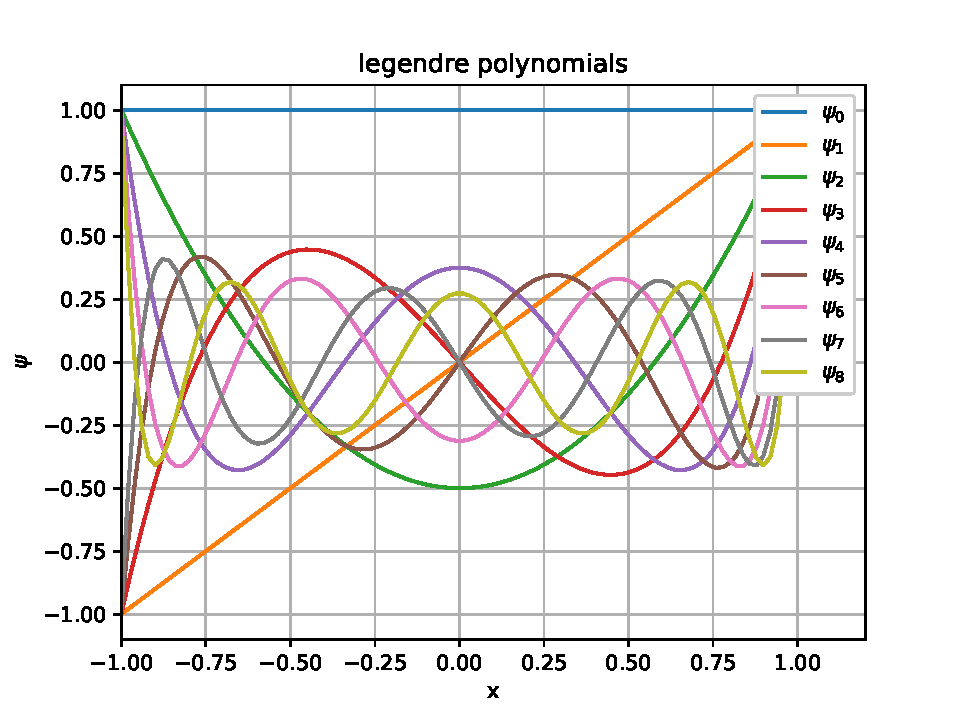
\includegraphics[width=0.8\textwidth]{Legendre.pdf}
		\caption{\label{Legendre} First $9$ Legendre polynomials}
	\end{center}
\end{figure}
Fig.\ref{Legendre} shows first $9$ Legendre polynomials. Observe that the `frequency' of the polynomials increases  (for increasing
count) indicating higher modes. Fig.\ref{Cheb} shows Chebyshev polynomials.
\begin{figure}[H]
	\begin{center}
		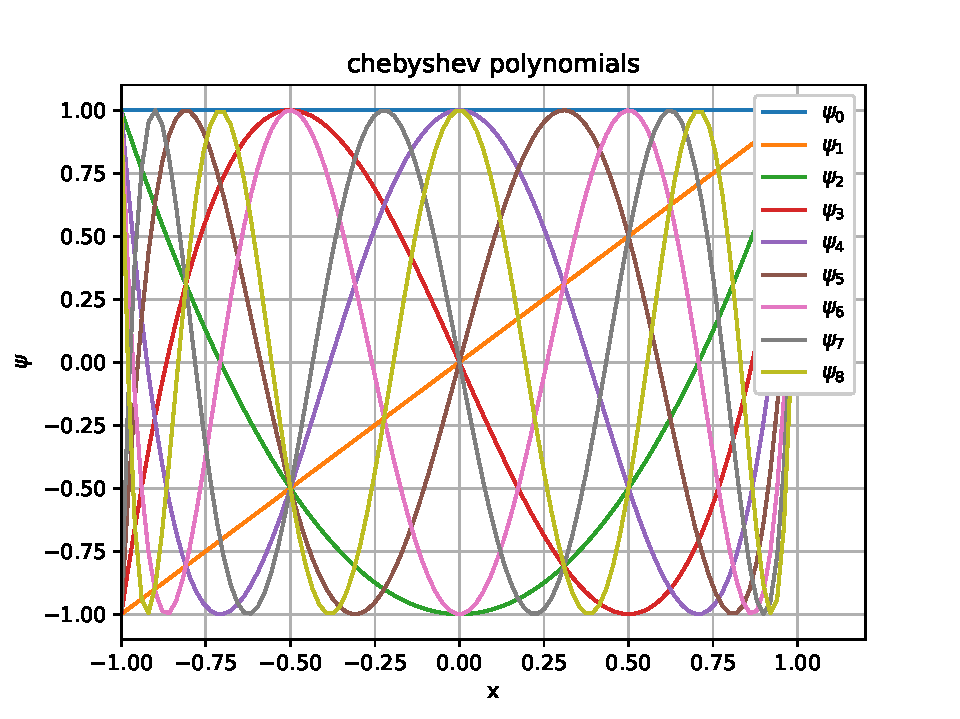
\includegraphics[width=0.8\textwidth]{Chebyshev.pdf}
		\caption{\label{Cheb} First $9$ Chebyshev polynomials}
	\end{center}
\end{figure}
\noindent The $1$D modal functions are implemented in:
\begin{verbatim}
FunctionalSpace::monomials1D(args),  
FunctionalSpace::legendrePolynomial1D(args), 
FunctionalSpace::chebyshevPolynomial1D(args) and 
FunctionalSpace::jacobiPolynomial1D(args)
\end{verbatim}
It is indeed difficult to comprehend how the polynomials shown in Fig.\ref{Legendre} and Fig.\ref{Cheb} be `orthogonal'.
The main reason for this is that we try to stick to our understanding of the $3$D space and the notion of 
orthogonality that comes with it, however, the polynomial space is essentially $\infty$ dimensional space. For
this space, the definition of orthogonality depends on the definition of the Inner-Product and `metric' of that space.
For $L^2$ space, the orthogonality is defined as,
\begin{equation}
	\int_{\Omega} \psi_i \psi_j d\Omega = \alpha \delta_{ij}, \hspace{4mm}\forall \psi_i, \psi_j \in L^2\{\Omega\} ~\& ~\alpha \in \mathbb{R}
\end{equation}
where, $\delta_{ij}$ is a `Kronecker Delta' which means $\delta_{ij} = 1 $ if $i=j$ and $0$ otherwise.
The functions $\psi_i$ and $\psi_j$ are orthonormal if $\alpha = 1$.


\subsection{Nodal Basis Functions}
The `nodal' basis functions are the set of functions which are `Cardinal' in nature. What that means is, at the
interpolation point, the basis function will have value $1$ and for all other collocation points, the value of the 
basis function will be zero. Thus, the interpolated value of the function agrees perfectly at the collocation points
but may have some error at other places. 
The general symbol used for nodal basis functions is $\phi$.
The interpolation itself is given as,
\begin{equation}
	f^N(x) = \sum_{i=0}^{N-1} f(x_i) \phi_i(x), \hspace{4mm} x \in C^0[a,b]
\end{equation}
and, $\phi_i(x_j) = \delta_{ij}$.
We use Lagrange polynomials as the nodal basis functions. The polynomials in $1$D are give as,
\begin{equation}
	\phi_i(x) = \prod_{j=0 , j \ne i}^{N-1} \frac{(x-x_j)}{(x_i - x_j)}
\end{equation}
it is clear that at $x=x_i$, $\phi_i(x_i) = 1$.
One crucial point that needs to be taken care of is selection of the collocation points $\left[x_0, x_1, ..., x_{N-1}\right]$.
It is seen that the equi-spaced arrangement of collocation points gives poor interpolation for very high orders of 
accuracies. Therefore we take these points as roots of orthonormal modal polynomials.
Popular choices for collocation points are Gauss-Legendre (LG) collocation points, Legendre-Gauss-Lobatto (LGL) points
or Chebyshev points. An important distinction between LG and LGL points is that, LGL points include the `end-points' 
whereas LG points include only the internal points. For DG methods, this doesn't have a significant difference since 
solving a Riemann problem at the face remains unchanged.

\subsection{Multidimensional Interpolation}
For number of dimensions greater than $1$, the interpolating polynomials are obtained depending on the type of the
element we wish to interpolate on. For hex elements, these are obtained using tensor product of $1$D polynomials.
i.e. 
\begin{equation}
	\phi(x,y,z) = \phi_{1D}(x)  \phi_{1D}(y)  \phi_{1D}(z)
\end{equation}
Whereas, for other types of elements, special multidimensional polynomials are used. However, the concept of 
modal and nodal basis functions remains essentially the same irrespective of the number of dimensions.
